\documentclass[14pt]{extarticle}
\usepackage[margin=1in]{geometry}
\usepackage{verbatim}
\usepackage{times}
\usepackage{graphicx}
\usepackage{float}

\begin{document}
\title{Big Data Assignment 2: Hadoop MapReduce Experimentation}
\author{Lee Boyd \\
        Corey Crosser \\
        Sean Soderman
        }
\date{\today}
\maketitle

\section{Notice}
We refer to Problem 4 as "part A" and Problem 5 as "part B".

%TODO: Need graphs in preferably pdf format
\section{Performance graphs}

\begin{figure}[H]
\centering
\includegraphics[width=5.2in]{bargraph.png}
\caption{}
\end{figure}


\section{Jobtracker Jobs}
\begin{figure}[H]
\centering
\includegraphics[width=5.2in]{JT.png}
\caption{}
\end{figure}


\section{Console Output}
\begin{figure}[H]
\centering
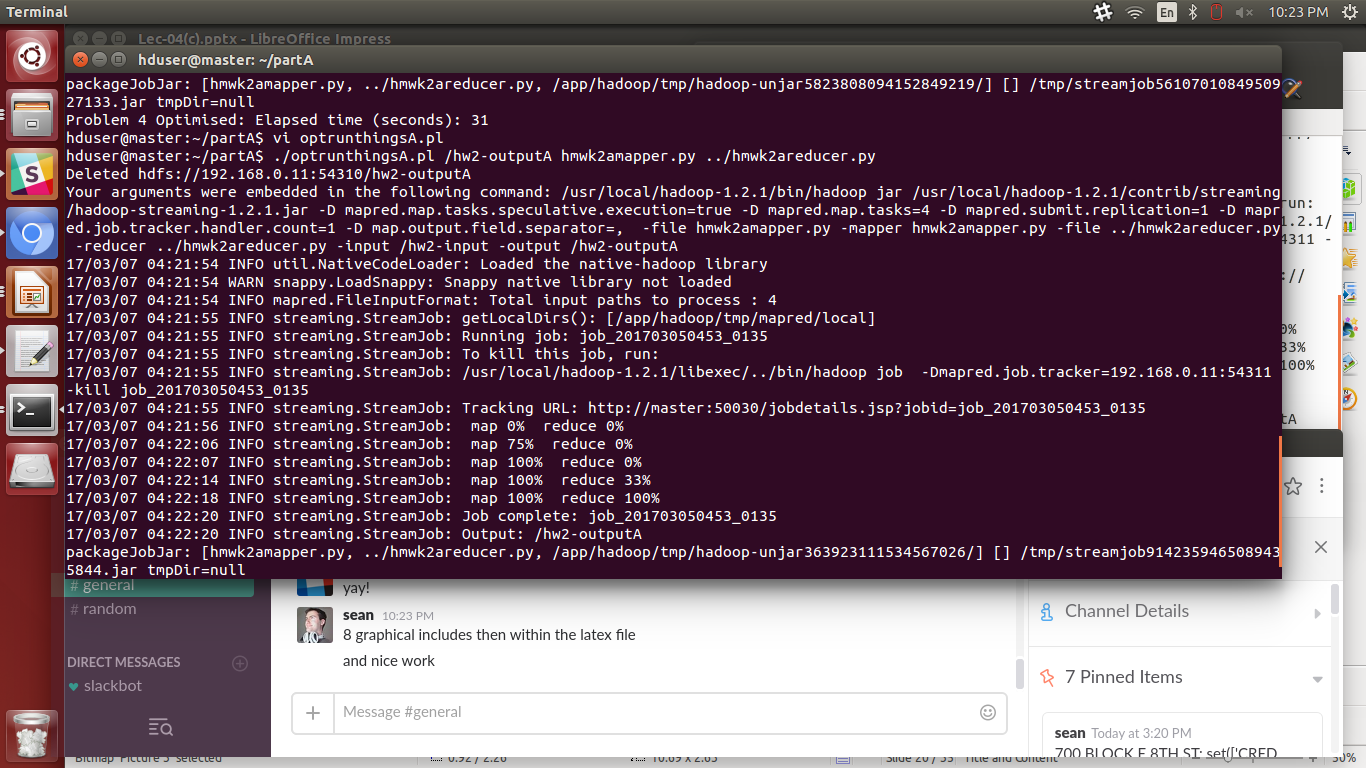
\includegraphics[width=5.2in]{consolescrnshot.png}
\caption{}
\end{figure}

\section{Work Division}
Sean handled the server setup and wrote Perl scripts to ease the formation of relevant MapReduce jobs.
Corey wrote the pseudocode for the mapping and reducing algorithms, including outputs and inputs.
Lee translated these algorithms to their Python form and emulated mapreduce for validation and verification. 
We all worked on finding optimization parameters for both parts of the assignment. 

\section{Performance Description}
%TODO
Using the combiner in Part 2 reduced the shuffle bytes from 32M to 88K, which
would make a significant performance impact in a real network.

Master as slave was the first optimization, where we used the master node as a slave node.  This is helpful, because it gives our mappers more horsepower in handling the data, and fits nicely with the scheme of having a mapper for every file, giving us four mappers and four slots.\\ 

We use speculative execution as a safeguard in case the master is slow with much of its memory allocated for other tasks such as jobtracker, we want to make sure that if it doesn't finish in a reasonable amount of time, then the other node can start to help it.  This safeguard would be more useful at a larger scale, where it would be more likely one of the other nodes would finish with their tasks before the master.  The small size of the task was also ideal for this optimization. \\

We use a combiner in part B, since the data is structured the same for the output of the mapper and reducer.  This optimization allows much of the work of putting similar key's values together locally to cut down on network traffic.  This is apparent in the statistics provided for the difference in shuffle, which would be more obvious on a larger problem. 
\\

We drop the mappers down to 3 on part B when using the combiner, with the assumption that more data locally is better, since the combiner would have more to move together and reduce network traffic significantly.  The shuffle cost was not as apparent here, but making sure local combiners have plenty to work with by giving the mapper as much as it can handle on a large scale is important for optimizing the combiner.

\end{document}
